%%%%% TODO %%%%%

% 1. Authors: Matt G, Jaclyn C, Matt T, others?
% 2. Correct values in `Manual updates' to those in the spawn intensity table
% 3. Author email(s) and/or phone number(s) required?

%%%%% Preamble %%%%%

% Set document style and font size
\documentclass[12pt]{article}

% Custom DFO Technical Reports
\usepackage{techreport}  

% New definitions: Title, year, report number
% Put words in math mode to prevent case changes (i.e., species names)
\newcommand{\trTitle}{Calculating the spawn index for Pacific herring ($Clupea$ $pallasii$) in British Columbia, Canada}
\newcommand{\trYear}{2017}
\newcommand{\trReportNum}{XXXX}

% New difinitions: Author info
\newcommand{\trAuthALong}{Matthew H.~Grinnell}
\newcommand{\trAuthBLong}{Other Authors}
\newcommand{\trAuthABack}{Grinnell, M.\,H.}
\newcommand{\trAuthBBack}{Authors, O.}
\newcommand{\trAuthAEmail}{\texttt{Matthew.Grinnell@dfo-mpo.gc.ca}}
\newcommand{\trAuthBEmail}{\texttt{Other.Authors@dfo-mpo.gc.ca}}
\newcommand{\trAuthAPhone}{(250)~756.7055}
\newcommand{\trAuthBPhone}{(250)~765.XXXX}

% New definition: Address
\newcommand{\trAddy}{Fisheries and Oceans Canada\\
Science Branch, Pacific Region\\
Pacific Biological Station\\
3190 Hammond Bay Road\\
Nanaimo, BC \enskip V9T 6N7}

% New definition: Citation
\newcommand{\trReference}{
\begin{hangparas}{1em}{1}
\trAuthABack{} and \trAuthBBack{} \trYear{}. \trTitle{}. Can. Tech. Rep. Fish. Aquat. Sci. \trReportNum{}: \pageref{TRlastRoman}{} + \pageref{LastPage}{} p.
\end{hangparas}}

% Set document options
%\linenumbers  % For drafts
%\onehalfspacing  % For drafts

% Let it begin
\begin{document}

% Sections in capitals
\renewcommand\listfigurename{LIST OF FIGURES}
\renewcommand\listtablename{LIST OF TABLES}

% Footnote symbols in front matter
\renewcommand*{\thefootnote}{\fnsymbol{footnote}}

%%%% Front matter %%%%%

% Format the first few pages
\thispagestyle{fancyplain}
\noindent
\begin{flushleft}
\LARGE
\textbf{\trTitle{}}
\vfill
\Large
\trAuthALong{}, and \trAuthBLong{}
\vfill
\trAddy{}
\vfill
\trYear{}
\vfill
\LARGE
\textbf{Canadian Technical Report of\\
Fisheries and Aquatic Sciences \trReportNum{}}
\lfoot{
\includegraphics[height=7mm]{Document/LogoDFO.png}}
\cfoot{}
\rfoot{
\includegraphics[height=7mm]{Document/LogoCanada.jpg}}
\end{flushleft}
\clearpage
  % Cover page
\footnotesize
\lfoot{} \cfoot{\thepage} \rfoot{}
\thispagestyle{empty}
\begin{center}
\textbf{Canadian Technical Report of Fisheries and Aquatic Sciences}
\end{center}
\noindent
Technical reports contain scientific and technical information that contributes to existing knowledge but which is not normally appropriate for primary literature.
Technical reports are directed primarily toward a worldwide audience and have an international distribution.
No restriction is placed on subject matter and the series reflects the broad interests and policies of Fisheries and Oceans Canada, namely, fisheries and aquatic sciences.
\indent
\par
Technical reports may be cited as full publications.
The correct citation appears above the abstract of each report.
Each report is abstracted in the data base \emph{Aquatic Sciences and Fisheries Abstracts}.
\par
Technical reports are produced regionally but are numbered nationally.
Requests for individual reports will be filled by the issuing establishment listed on the front cover and title page.
Out-of-stock reports will be supplied for a fee by commercial agents.
\par
Numbers 1--456 in this series were issued as Technical Reports of the Fisheries Research Board of Canada.
Numbers 457--714 were issued as Department of the Environment, Fisheries and Marine Service, Research and Development Directorate Technical Reports.
Numbers 715--924 were issued as Department of Fisheries and Environment, Fisheries and Marine Service Technical Reports.
The current series name was changed with report number 925.
\bigskip
\begin{center}
\textbf{Rapport technique canadien des sciences halieutiques et aquatiques}
\end{center}
\noindent
Les rapports techniques contiennent des renseignements scientifiques et techniques qui constituent une contribution aux connaissances actuelles, mais qui ne sont pas normalement appropri�s pour la publication dans un journal scientifique.
Les rapports techniques sont destin�s essentiellement � un public international et ils sont distribu�s � cet �chelon.
II n'y a aucune restriction quant au sujet; de fait, la s�rie refl�te la vaste gamme des int�r�ts et des politiques de P�ches et Oc�ans Canada, c'est-�-dire les sciences halieutiques et aquatiques.
\indent
\par
Les rapports techniques peuvent �tre cit�s comme des publications � part enti�re.
Le titre exact figure au-dessus du r�sum� de chaque rapport.
Les rapports techniques sont r�sum�s dans la base de donn�es \emph{R�sum�s des sciences aquatiques et halieutiques}.
\par
Les rapports techniques sont produits � l'�chelon r�gional, mais num�rot�s � l'�chelon national.
Les demandes de rapports seront satisfaites par l'�tablissement auteur dont le nom figure sur la couverture et la page du titre.
Les rapports �puis�s seront fournis contre r�tribution par les agents commerciaux.
\par
Les num�ros 1 � 456 de cette s�rie ont �t� publi�s � titre de Rapports techniques de l'Office des recherches sur les p�cheries du Canada.
Les num�ros 457 � 714 sont parus � titre de Rapports techniques de la Direction g�n�rale de la recherche et du d�veloppement, Service des p�ches et de la mer, minist�re de l'Environnement.
Les num�ros 715 � 924 ont �t� publi�s � titre de Rapports techniques du Service des p�ches et de la mer, minist�re des P�ches et de l'Environnement.
Le nom actuel de la s�rie a �t� �tabli lors de la parution du num�ro 925.
\clearpage
  % Tech report page
\normalsize
\pagenumbering{roman}
\thispagestyle{empty}
\noindent
\begin{center}
Canadian Technical Report of\\
Fisheries and Aquatic Sciences \trReportNum{}
\vfill
\trYear{}
\vfill
\MakeTextUppercase{\trTitle{}}
\vfill
by
\vfill
\trAuthALong{},\footnote{E-mail: \trAuthAEmail{} $|$ telephone: \trAuthAPhone{}} and \trAuthBLong{}\footnote{E-mail: \trAuthBEmail{} $|$ telephone: \trAuthBPhone{}}
\vfill
\trAddy{}
\end{center}
\clearpage
  % Inside cover page
\vspace*{\fill}
\begin{center}
\begin{minipage}{\widthof{\copyright{} Her Majesty the Queen in Right of Canada, \trYear{}}}
\copyright{} Her Majesty the Queen in Right of Canada, \trYear{}\\
Cat. No. Fs97-6/\trReportNum{} E \hfill ISSN 0706-6457\\
Cat. No. Fs97-6/\trReportNum{} E-PDF \hfill ISSN 1488-5379
\end{minipage}
\end{center}
\par
\bigskip
\noindent
Correct citation for this publication:
\bigskip
\par
\begin{hangparas}{1em}{1}
\trReference{}
\end{hangparas}
\clearpage
  % Colophon page
\tableofcontents \clearpage  % Table of contents page
%\listoffigures \listoftables \clearpage  % Lists of figures and tables (optional)
\noindent
\section*{ABSTRACT}
\addcontentsline{toc}{section}{ABSTRACT}
\trReference{}
\bigskip
This report documents the calculations used to convert spawn survey observations (e.g., number of egg layers, extent of spawn) to the spawn index for Pacific herring ($Clupea$ $pallasii$) in British Columbia (BC), Canada.
There are three types of spawn survey observations: surface observations, underwater observations of spawn on Macrocystis, and underwater observations of spawn on understory.
Data from these three survey types are combined to develop an overall annual spawn index for each stock assessment region in BC.
The spawn index is one component of Pacific herring stock assessments in BC.
Note that the 'spawn index' is not scaled by the spawn survey scaling parameter, $q$ and therefore is not an estimate of spawning stock biomass.
\section*{R\'{E}SUM\'{E}}
\addcontentsline{toc}{section}{R\'{E}SUM\'{E}}
\trReference{}
\bigskip
Ceci est la r�sum�...
\vfill
\label{TRlastRoman}
\clearpage
  % Abstact and resume page

% Settings for the main document
\pagenumbering{arabic}  % Regular page numbers
\thispagestyle{empty}  % No page number on first page
\renewcommand*{\thefootnote}{\arabic{footnote}}  % Back to numeric footnotes
\setcounter{footnote}{0}  % And start at 1

%%%%% Main document %%%%%

\section{INTRODUCTION}

This report describes the calculations used to convert spawn survey observations (e.g., number of egg layers, extent of spawn) to the spawn index for Pacific herring (\!\emph{Clupea pallasii}) in British Columbia (BC), Canada.
Note that the `spawn index' is not scaled by the spawn survey scaling parameter, $q$ \citeyearpar[CSAS][]{CSAS2015b}, and is therefore not an estimate of spawning stock biomass.
The spawn index is one component of BC herring stock assessments.

Spawn surveys collect the data used to calculate the spawn index.
There are three types of spawn survey observations: surface survey observations, underwater observations of spawn on Macrocystis, and underwater observations of spawn on understory.
Understory observations have two components: spawn on the bottom, and spawn on vegetation (i.e., algae).
Surface spawn surveys have the coarsest spatial resolution and greatest spatial extent of the three survey types (Ref?).
Surface spawn surveys were the only survey type prior to 1988, and they are still used extensively for minor spawns because they are adequate for narrow spawns in shallow water (Ref?).
Macrocystis and understory spawn surveys are conducted using SCUBA gear.
Underwater SCUBA surveys have been used for all major spawns since 1988, and are thought to be more accurate than surface spawn surveys (Ref?).
Herring spawn surveys began in 1928, but are considered incomplete prior to 1937 because many potential areas were not surveyed (Ref?).

Herring spawn survey observations have a nested hierarchical structure: quadrats are nested within transects, transects are nested within spawns, and spawns are nested within locations.
For stock assessment purposes, locations are nested within sections, sections are nested within statistical areas, and statistical areas are nested within five major and two minor stock assessment regions (SARs) in BC.
The major SARs are Haida Gwaii, Prince Rupert District, Central Coast, Strait of Georgia, and West Coast Vancouver Island; the minor SARs are Area 27, and Area 2 West (Figure \ref{figBC}).
Another level of data structure is `beds', which are habitat features as opposed to distinct spatial areas.
Bed widths are used to calculate the spawn index for surface surveys.

\begin{figure}
\centering
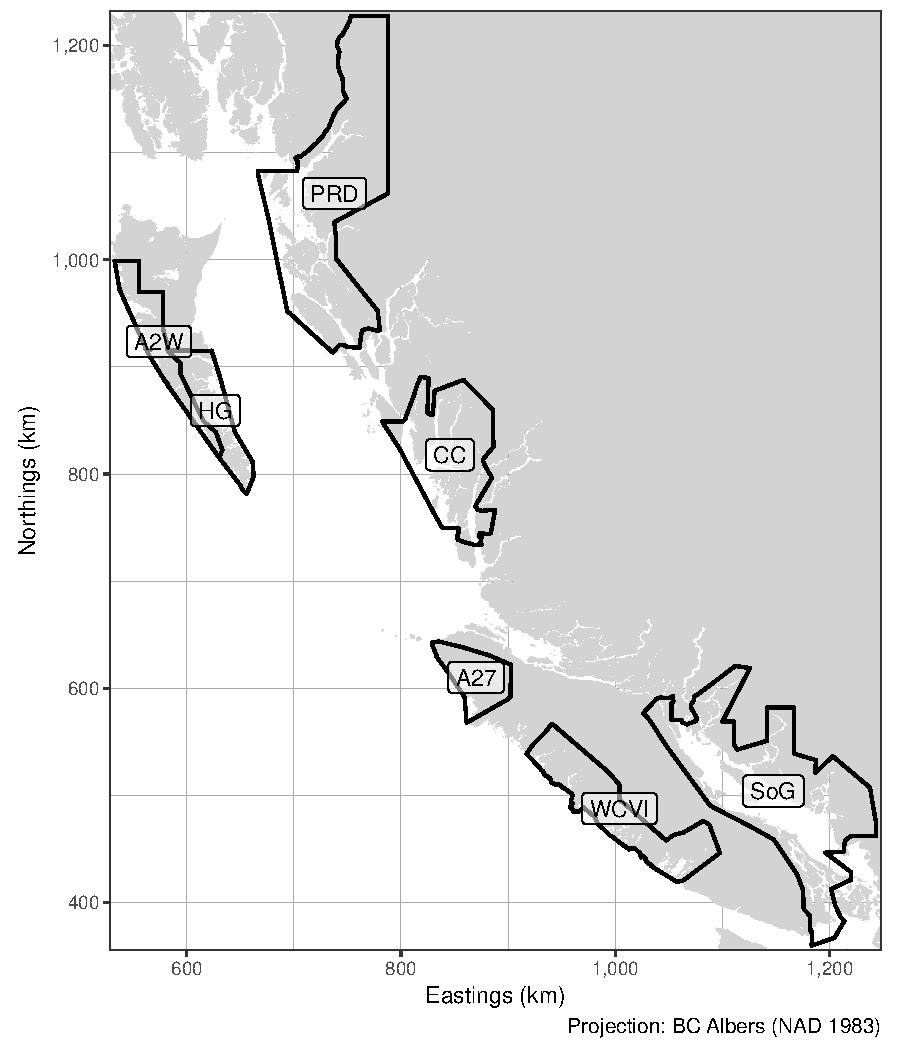
\includegraphics[width=\linewidth]{Figures/BC.pdf}
\caption[Boundaries for British Columbia Pacific herring stock assessment regions (SARs)]
{Boundaries for British Columbia Pacific herring stock assessment regions (SARs): there are five major SARs (Haida Gwaii, HG; Prince Rupert District, PRD; Central Coast, CC; Strait of Georgia, SoG; and West Coast Vancouver Island, WCVI), and two minor SARs (Area 27, A27; and Area 2 West, A2W).}
\label{figBC}
\end{figure}

We use the \textbf{R} \citeyearpar[RCT][]{R-3.3.2} script \texttt{Spawn.R} to calculate the spawn index.
The script pulls data from the spawn database (Ref?), and does the calculations described in the following sections.
Note that variable names in this document correspond to variable names in the \texttt{Spawn.R} script.

\section{FECUNDITY}

Female Pacific herring produce an average of 200 eggs per gram, g of total body weight \citep{Hay1985}.
We assume that females account for 50\% of spawners, and we use the following fecundity conversion factor for eggs to tonnes, t, of spawners
\begin{equation}
\frac {1 \cdot 10^{8}~\text{eggs}} {\text{t}} = \frac{200~\text{eggs}} {\text{g}} \times 0.5 \times \frac{1 \cdot 10^{6}~\text{g}} {\text{t}} \enspace .
\label{eqFecundityConv}
\end{equation}
%Therefore, we divide eggs by $1 \cdot 10^{8}$ to determine spawning biomass in tonnes.
%In order to avoid precision loss with large numbers -- is that the reason?
Note that we report eggs in thousands (i.e., $\text{eggs} \cdot 10^{3}$) in the \textbf{R} script, and correspondingly in this report.
Therefore, we divide $\text{eggs} \cdot 10^{3}$ by $1 \cdot 10^{5}$ to determine spawning biomass in tonnes.

\section{SURFACE SPAWN}

Surface spawn surveys collect data along transects, and we calculate spawn metrics at the transect, and spawn/bed level.

\subsection{TRANSECT LEVEL CALCULATIONS}

For each bottom type, egg layers is
\begin{equation}
EggLyrs = Layers \times Proportion
\label{eqEggLayersSurf}
\end{equation}
where $Layers$ is the number of egg layers on a given bottom type, and $Proportion$ is the proportion of the transect covered by the bottom type.
At the transect level, the sum of $EggLyrs$ is $EggLyrsTotT$.
That is to say, $EggLyrsTotT$ is the sum of $EggLyrs$ for all the bottom types within a given transect.
For the time period when `Intensity' categories were recorded instead of estimating the number of egg layers, intensity is converted to $EggLyrsTotT$ (Table \ref{tabIntensity}).
Surface egg density in thousands is \citep{SchweigertEtal1997}%
\footnote{Notwithstanding the units provided in \citet{SchweigertEtal1997}, surface egg density is in thousands ($\text{eggs} \cdot 10^{3} \cdot \text{m}^{-2}$; J.~Schweigert, personal communication, 24 February 2017).}
\begin{equation}
EggDensT = EggLyrsTotT \times 212.218 + 14.698
\label{eqEggDensSurf}
\end{equation}
where $EggDensT$ is in $\text{Eggs} \cdot 10^{3} \cdot \text{m}^{-2}$. 

\begin{table}
\centering
\caption[Spawn intensity categories and associated egg layers for Pacific herring surface spawn surveys]
{Spawn intensity categories and associated egg layers for Pacific herring surface spawn surveys for the periods 1928--1950, and 1951--1978 (Ref?).
Note that the survey protocol was updated from five to nine intensity categories in 1951.}
\begin{tabular}{ccr}
\toprule
\multicolumn{2}{c}{Intensity category} & \\
1928--1950 & 1951--1978 & Egg layers\\
\midrule
0 & 0 & 0.0000 \\
1 & 1 & 0.5529 \\
 & 2 & 0.9444 \\
2 & 3 & 1.3360 \\
 & 4 & 2.1496 \\
3 & 5 & 2.9633 \\
 & 6 & 4.1318 \\
4 & 7 & 5.3002 \\
 & 8 & 6.5647 \\
5 & 9 & 7.8291 \\
\bottomrule
\end{tabular}
\label{tabIntensity}
\end{table}

\subsection{SPAWN/BED LEVEL CALCULATIONS}

At the spawn/bed level, the mean of $EggDensT$ is $EggDensMeanS$.
Two other metrics are required at the spawn/bed level: the spawn/bed length $Length$ and width $WidthS$, both in metres.
We set $WidthS$ to the first non-missing value from the bed width, section width, region width, or observed width (in that order).
The surface spawn index is
\begin{equation}
SurfSI = \frac{EggDensMeanS \times Length \times WidthS} {1 \cdot 10^{5}}
\label{eqBiomassSurf}
\end{equation}
where $SurfSI$ is in tonnes, based on Equation \ref{eqFecundityConv}.

\subsection{MANUAL CORRECTIONS}

To correct errors in the surface spawn database, we make \ref{enumLast} manual updates to $EggLyrsTotT$ for the following records (J.~Schweigert, personal communication, 21 February 2017):
\begin{enumerate}
\item Update $EggLyrsTotT$ to 2.15 for the 15 records in the year 1979, statistical area 2, and with intensity 4;
\item Update $EggLyrsTotT$ to 0.5529 for the 1 record in the year 1962, statistical area 14, and with intensity 0;
\item Update $EggLyrsTotT$ to 0.55 for the 4 records in the year 1981, statistical area 24, and with $EggLyrsTotT = 0$;
\item Update $EggLyrsTotT$ to 1.34 for the 7 records in the year 1982, statistical area 23, and with intensity 3;
\item Update $EggLyrsTotT$ to 2.33 for the 41 records in the year 1984, statistical area 24, and with intensity 0; and
\item Update $EggLyrsTotT$ to 2.98 for the 14 records in the year 1982, statistical area 27, and with $EggLyrsTotT = 0$. \label{enumLast}
\end{enumerate}

\section{MACROCYSTIS SPAWN}

Macrocystis spawn surveys collect data for individual plants, and we calculate spawn metrics at the transect, and spawn levels.

\subsection{TRANSECT LEVEL CALCULATIONS}

Several metrics are collected at the transect level: transect length $LengthT$, transect width $WidthT$, and Macrocystis length $LengthMacroT$, all in metres, as well as transect area $AreaT$, in square metres.
The `Macrocystis length' is the distance that the Macrocystis extends perpendicular to the shore (?).
Note that $LengthT$ and $LengthMacroT$ will be the same if there is no recorded Macrocystis bed length.
In addition, we calculate metrics for mature Macrocystis plants: mean height $HeightMeanT$ in metres, mean egg layers $LayersMeanT$, total number of fronds $FrondsTotT$, and total number of plants $PlantsTotT$.

\subsection{SPAWN LEVEL CALCULATIONS}

At the spawn level, the mean of $LengthMacroT$ is $LengthMacroMeanS$, the mean of $LengthT$ is $LengthMeanS$, and the sum of $AreaT$ is $AreaTotS$, all in metres.
In addition, the sum of $PlantsTotT$ is $PlantsTotS$, the sum of $FrondsTotT$ is $FrontsTotS$, the mean of $HeightMeanT$ is $HeightMeanS$, and the mean of $LayersMeanT$ is $LayersMeanS$. 
The number of fronds per plant is
\begin{equation}
FrondsPerPlantS = \frac{FrondsTotS} {PlantsTotS} \, .
\label{eqFrondsPerPlant}
\end{equation}
The number of eggs per plant in thousands is \citep{HaegeleSchweigert1990}
\begin{multline}
EggsPerPlantS = 0.073 \times LayersMeanS^{0.673} \times \\ 
HeightMeanS^{0.932} \times FrondsPerPlantS^{0.703} \times 1 \cdot 10^{3}
\label{eqEggsPerPlantMacro}
\end{multline}
where $EggsPerPlantS$ is in $\text{Eggs} \cdot 10^{3} \cdot \text{plant}^{-1}$. 
Macrocystis egg density in thousands is
\begin{equation}
EggDensS = \frac{EggsPerPlantS \times PlantsTotS} {AreaTotS}
\label{eqEggDensityMacro}
\end{equation}
where $EggDenS$ is in $\text{Eggs} \cdot 10^{3} \cdot \text{m}^{-2}$.
The Macrocystis spawn index is
\begin{equation}
MacroSI = \frac{EggDensS \times LengthMacroMeanS \times LengthMeanS} {1 \cdot 10^{5}}
\label{eqBiomassMacro}
\end{equation}
where $MacroSI$ is in tonnes, based on Equation \ref{eqFecundityConv}.

\section{UNDERSTORY SPAWN}

Understory spawn surveys collect data in quadrats, and we calculate spawn metrics at the quadrat, transect, and spawn levels.
We calculate two separate estimates of egg density at the quadrat level: spawn on the bottom, and spawn on vegetation (i.e., algae).

\subsection{QUADRAT LEVEL CALCULATIONS}

Bottom egg density in thousands is \citep{HaegeleEtal1979}
\begin{equation}
EggsDBot = 340 \times BotLayers \times BotProp
\label{eqEggDensUnderB}
\end{equation}
where $BotLayers$ is the number of egg layers on the bottom, $BotProp$ is the proportion of the bottom covered in spawn, and $EggsDBot$ is in $\text{Eggs} \cdot 10^{3} \cdot \text{m}^{-2}$.
Vegetation egg density in thousands is \citep{Schweigert2005}
\begin{multline}
EggsDVeg = 600.567 \times VegLayers^{0.6355} \times VegProp^{1.413} \times V \times 1.0512
\label{eqEggDensUnderV}
\end{multline}
where $VegLayers$ is the number of egg layers on vegetation, $VegProp$ is the proportion of the bottom covered by the vegetation type, $V$ is the vegetation coefficient (Table \ref{tabVegTypes}), and $EggsDVeg$ is in $\text{Eggs} \cdot 10^{3} \cdot \text{m}^{-2}$.
The total linear weighted understory egg density in thousands is%
\footnote{Explain why we calculate weighted egg density, $EggDensWtQ$.
Is it because transects are different lengths (which we call widths)?}
\begin{equation}
EggDensWtQ = \left( EggsDBot + EggsDVeg \right) \times Width
\label{eqEggDensWtUnder}
\end{equation}
where $Width$ is the transect width in metres, and $EggDensWtQ$ is in $\text{Eggs} \cdot 10^{3} \cdot \text{m}^{-1}$.
Note that we expand $Width$ in certain years to account for footrope expansion when wet, if applicable.\footnote{We don't do this, so can we remove if from here, and the \textbf{R} script?}

\begin{table}
\centering
\caption[Vegetation (i.e., algae) types and coefficients for Pacific herring understory spawn surveys]
{Vegetation (i.e., algae) types and coefficients, $V$ for Pacific herring understory spawn surveys \citep{Schweigert2005}.}
\begin{tabular}{lr}
\toprule
Vegetation type & Coefficient, $V$\\
\midrule
Grasses & 0.9715 \\
Grunge & 1.0000 \\
Kelp, flat & 0.9119 \\
Kelp, standing & 1.1766 \\
Leafy algae & 0.6553 \\
Rockweed & 0.7793 \\
Sargassum & 1.1766 \\
Stringy algae & 1.0000 \\
\bottomrule
\end{tabular}
\label{tabVegTypes}
\end{table}

\subsection{TRANSECT LEVEL CALCULATIONS}

At the transect level, the mean $EggDensWtQ$ is $EggDensWtMeanT$.

\subsection{SPAWN LEVEL CALCULATIONS}

At the spawn level, the sum of transect widths $Width$ is $WidthTotS$, the mean of $Width$ is $WidthMeanS$, and the vegetation length is $VegLengthS$, all in metres.
The `vegetation length' is the distance that the vegetation extends perpendicular to the shore (?).
Note that $VegLength$ will be equal to the transect length if there is no recorded vegetation length.
The sum of $EggDensWtMeanT$ is $EggDensWtTotS$.
Understory egg density is 
\begin{equation}
EggDensWtS = \frac{EggDensWtTotS} {WidthTotS}
\label{eqEggDensityUnder}
\end{equation}
where $EggDensWtS$ is in $\text{Eggs} \cdot 10^{3} \cdot \text{m}^{-2}$.
The understory spawn index is
\begin{equation}
UnderSI = \frac{EggDensWtS \times VegLengthS \times WidthMeanS} {1 \cdot 10^{5}}
\label{eqBiomassUnder}
\end{equation}
where $UnderSI$ is in tonnes, based on Equation \ref{eqFecundityConv}.

\section{TOTAL SPAWN}

The total spawn index for each spawn is
\begin{equation}
TotalSI = SurfSI + MacroSI + UnderSI
\label{eqTotalSI}
\end{equation}
where $TotalSI$ is in tonnes.
As previously mentioned, the spawn index must be scaled by the spawn survey scaling parameter, $q$ \citeyearpar[CSAS][]{CSAS2015b} before it can be considered to be an estimate of spawning stock biomass.

\section{ACKNOWLEDGEMENTS}

People we may want to thank:
\begin{itemize}
\item Jake Schweigert for background and reasoning re the manual corrections
\end{itemize}

% References
\bibliographystyle{Document/CJFAS}
\addcontentsline{toc}{section}{\refname}\bibliography{Document/Grinnell}

% The end
\end{document}
